\documentclass{article} % Especially this!

\usepackage[english]{babel}
\usepackage[utf8]{inputenc}
\usepackage[margin=1.5in]{geometry}
\usepackage{amsmath}
\usepackage{amsthm}
\usepackage{amsfonts}
\usepackage{amssymb}
\usepackage{graphicx}
\usepackage{hyperref}
\usepackage[numbers, square]{natbib}
\usepackage{fancybox}
\usepackage{epsfig}
\usepackage{soul}
\usepackage[framemethod=tikz]{mdframed}
\usepackage[shortlabels]{enumitem}
\usepackage[version=4]{mhchem}
\usepackage{multicol}
\usepackage{graphicx}
\graphicspath{ {./} }

\newcommand{\blah}{blah blah blah \dots}

\setlength{\marginparwidth}{3.4cm}

\newcommand{\summary}[1]{
\begin{mdframed}[nobreak=true]
\begin{minipage}{\textwidth}
\vspace{0.5cm}
\end{minipage}
\end{mdframed}}

\renewcommand*{\thefootnote}{\fnsymbol{footnote}}

\title{
\normalfont \large
\textsc{ASSIGNMENT-1
\vspace{10pt}
\\COL 216, Spring 2021} \\
[10pt] 
\rule{\linewidth}{0.5pt} \\[6pt] 
\Large Area Under Curve using MIPS \\
\rule{\linewidth}{2pt}  \\[10pt]
}
\author{Jitender Kumar Yadav, 2019CS10361
\\Asha Ram Meena, 2019CS10337}
\date{\normalsize February 23, 2021}
\begin{document}

\maketitle
\section{Problem Statement}
\textbf{Write a MIPS Assembly Program for obtaining the area under a curve formed by joining successive points by a straight line.}

\section{Algorithm and Approach}
If we join two points by a straight line, the area between the points and the x-axis is essentially a trapezium if the points lie on the same side of the x-axis, with area given by:
\[\Delta = \left | \frac{1}{2} \times (x_2 - x_1) \times (y_2 + y_1)\right | \]
If the points lie on the opposite sides of the axis, the area has to be calculated by considering the triangles which can be found using the following formula:
\[\Delta = \frac{1}{2} \times \left | \frac{x_2 - x_1}{y_2 - y_1} \right | \times (y_1 \times y_1 + y_2 \times y_2)\]
The following steps are used to calculate the area:
\begin{itemize}
    \item[$\diamond$] The integer n is read.
    \item[$\diamond$] The pair (x,y) are read one by one starting from first point till the last.
    \item[$\diamond$] When the k\textsuperscript{th} pair is read for $k > 1$, two registers store the current and the previous coordinates.
    \item[$\diamond$] The calculation of area between the current and previous points is done by using the above formula, by use of conditional statements. This area is added to the value of variable representing current area.
    \item[$\diamond$] The value of area at the end of all iterations in returned and printed.
\end{itemize}

\section{Input and Output}
The input is to be taken from the user using console and the output shall be printed on the console itself.
\subsection{Input Specifications:}
\begin{itemize}
    \item The first line inputs an integer n, the number of points.
    \item The next 2n lines input the x- and y- co-ordinates of the n points one after the other for each point.
    \item It is assumed that $\left|x_i\right| \leq 2^{15}$ and $\left|y_i\right| \leq 2^{15}$, $1 \leq i \leq n$ where $x_i$ and $y_i$ represent the x- and y-coordinates of $i^{th}$ point.
\end{itemize}
\subsection{Output}
\begin{itemize}
    \item The output is calculated and shown at the end after the input has been read and processed.
\end{itemize}
\subsection{Sample I/O}
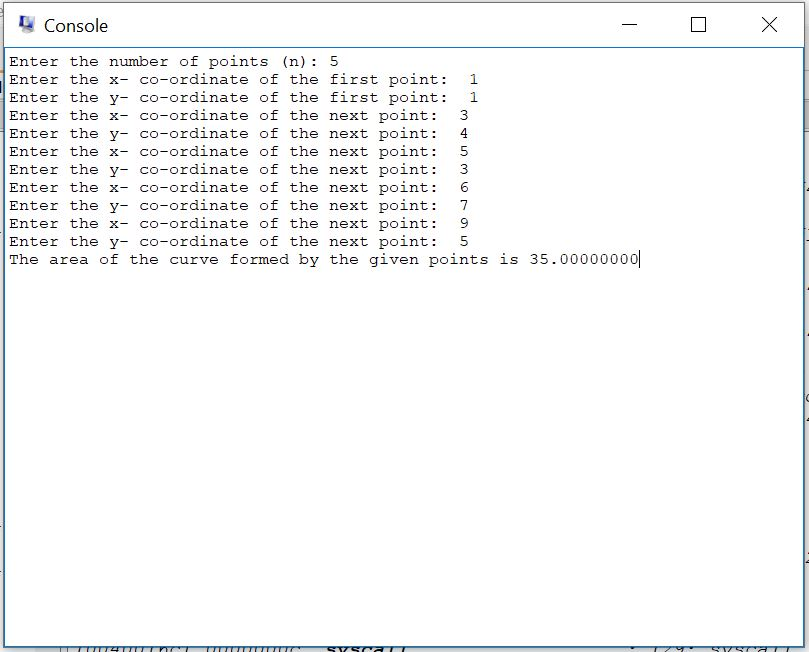
\includegraphics{sampleio_A1.JPG}

\section{The Code}
\subsection{Registers}
\begin{itemize}
    \item \textbf{\$s0} : stores the number of points, n
    \item \textbf{\$t1} : stores the x-coordinate of previous point
    \item \textbf{\$t2} : stores the y-coordinate of previous point or its absolute value
    \item \textbf{\$t3} : stores the iterator i to loop over n points
    \item \textbf{\$t6} : stores the x-coordinate of current point
    \item \textbf{\$t7} : stores the y-coordinate of current point or its absolute value
    \item \textbf{\$t8} : stores the value of width of the trapezium ($x_2 - x_1$)
    \item \textbf{\$t9} : stores the signed y-coordinate of the current point to be stored later in \$t2
    \item \textbf{\$t4} : stores the numerator of the area under the current line segment
    \item \textbf{\$t5} : stores the denominator of the area under the current line segment
    \item \textbf{\$f1} : stores the total area till the last point
    \item \textbf{\$f2} : stores the float value of the numerator in current expression of area
    \item \textbf{\$f3} : stores the float value of the denominator in current expression of area
    \item \textbf{\$f4} : stores the area under the line segment joining the current and previous points
\end{itemize}
\subsection{Location Labels}
\begin{itemize}
    \item \textbf{loop} : compares the value of i against n and thus inputs current point, transferring it to the correct area calculation function
    \item \textbf{findArea} : calculates and adds the current area to the total area register
    \item \textbf{pos\_neg} : calculates the numerator and denominators for the current area when points are on the opposite sides
    \item \textbf{printArea} : prints the area to the console
\end{itemize}

\section{Testing}
Some test-cases were generated by a random number generator and their output was evaluated by using a python 3.0 program. While the test-cases to consider the corner cases were hand-made and evaluated.
\\The test cases are stored in files A1\_Test1.in to A1\_Test8.in and the outputs are auto-generated by a python file checker.py and stored in A1\_Test\_out.out in the same folder.
\\The code was tested with all 8 sample testcases as well as new random test cases and the final area was manually calculated. The final area came out to be the same as expected, thus validating the code stored in the file "A1\_area.asm".
\end{document}